\chapter{Team 5 Agent Design}\label{team_5_agent_design}

The Team 5 agent operates on the basis that upon entering the tower, the need to ensure its own survival is its only aim and therefore the agent should maximise its own HP whenever given the opportunity to do so. When there is not enough food to fully satisfy all agents, the agent alters its behaviour to best increase its long-term survival.

This situation can be thought of as a `hawk-dove' game where it is beneficial for all agents to take less food but any single agent who does so is worse off if no other agents follow suit. Communication is key to breaking out of this situation. This agent will attempt to establish relationships with surrounding agents -- the agent has parameters to judge other agents and also attempts to learn about the tower -- and encourage behaviours that benefit the overall tower utility.

However, the agent will also be influneced by the behaviour of agents around it: if other agents are selfish then it will also be selfish. This can be thought of as a `tit-for-tat' strategy, but with enough HP, agents will be willing to `make the first move', with the insurance that if others do not follow then they have some buffer time to re-establish their own selfish behaviour.

An agent will maintain a low HP only if it is confident that other agents will allow it to survive by leaving enough food, through the signing of treaties to build trust. A tower that consists solely of Team 5 agents would require those at the top to be willing to decrease their own short-term satisfaction in order to give the best chance of survival for all agents, and trust others to do the same upon reshuffling.

Section \ref{sec:team5-overview} provides an overview of the agent's parameters and strategy, Section \ref{sec:team5-messaging} describes the agent's communication strategy, Section \ref{sec:team5-memory} describes how the agent stores its social network and how it judges other agents, and Section \ref{sec:team5-treaties} describes how the Team 5 agent utilises treaties. Finally, Section \ref{sec:team5-experimentation} contains analysis of this agent and how it performs in a Tower consisting of itself alone and together with other agent types and Section \ref{sec:team5-conclusion} provides summarising remarks regarding the implementation of this agent type.

\section{Agent Overview}
\label{sec:team5-overview}

\ToDo{Give better description of Run function}

The strategy employed by this agent aims to maximise its chances of survival while also considering those who have helped the agent in the past.

At the beginning of each day, the agent's `personality' is updated using various parameters stored from previous days. These personality parameters are shown in Table \ref{tab:team5-personality}.

\begin{table}
    \centering
\begin{tabular}%
    {| >{\raggedleft\arraybackslash}p{0.25\linewidth} | %
    >{\raggedright\arraybackslash}p{0.65\linewidth} | %
    }
    \hline
    Selfishness          & Ranges from 0 to 10. Determines how much the agent will act for their own survival as opposed to the best interests of the surrounding agents\\
    \hline
    Last Meal            & How much the agent ate in their last meal\\
    \hline
    Days Since Last Meal & How many days since the agent last ate\\
    \hline
    % HP After Eating      & \\
    % \hline
    Aim HP               & Defines the goal HP the agent would like to reach at the end of the day\\
    \hline
    Attempt Food         & The amount of food the agent will attempt to take from the platform\\
    \hline
    Messaging Counter    & Determines which message type to send to which floor \\
    % \hline
    % Treaty Send Counter  & \\
    % \hline
    % Attempt To Eat       & \\
    % \hline
    Leadership           & A threshold value required for the agent to propose treaties\\
    \hline
    Social Memory        & Stores the information the agent learns about other agents, as well as its opinion of them (see Table \ref{tab:team5-memory})\\
    \hline
    Surrounding Agents   & A list of the agent's neighbours\\
    \hline
\end{tabular}
\caption{The personality parameters of Team 5's agent}
\label{tab:team5-personality}
\end{table}

At the start of each tick, the agent checks to see if it has received any messages and if so, will respond to these\footnote{Note that an agent can receive and respond to only one message per tick.}. The agent then sends out messages to other agents. The mechanism for messaging is described in Section \ref{sec:team5-messaging}.

\section{Messaging}\label{sec:team5-messaging}
Collaboration between different agents operating in a system requires communication. The motivation for messaging is to improve the agent's understanding of its surroundings, enable building of mutually beneficial relationships, and introduce collaboration and argeement between parties.

\subsection*{Strategy}\label{sec:team5-messaging-strategy}
The agent's approach to messaging is to adopt a ``passive observer'' role focussed on gathering information about other agents to organise itself with these agents in the tower. With more information at its disposal, the agent can make more informed decisions to balance its own individual utility with the collective utility of the agents in the tower.

\ToDo{choose whether to say 12 or 8 ticks to send all messages}
The agent sends three types of messages targeting each of the agents two floors above and below its own floor; it therefore takes 12 ticks to send all of its messages. These messages ask for the HP, intended food intake, and actual food intake of other agents. The decision of which message type to send to which floor is controlled by the Messaging Counter described in Table \ref{tab:team5-personality}. This counter is incremented each tick, and reset either every 25 ticks or at the end of each day, whichever comes first. This ensures that the agent is requesting up-to-date information regularly for use in its decision making.

The order of sent messages is:
\begin{enumerate}
    \item Ask for an agent's HP
    \item Ask for an agent's previous food intake
    % \item Ask for an agent's intended food intake
\end{enumerate}
The Team 5 agent first targets the agent immediately below it, then the agent immediately above, then two floors below, and finally the agent two floors above.

\section{Social Memory}\label{sec:team5-memory}
The agent stores the information gained from communication in its `memory': the information stored by this data structure is shown in Table \ref{tab:team5-memory}.

\begin{table}
    \centering
    \begin{tabular}%
        {| >{\raggedleft\arraybackslash}p{0.25\linewidth} | %
        >{\raggedright\arraybackslash}p{0.65\linewidth} | %
        }
        \hline
        Agent ID & An agent's unique ID\\
        \hline
        Agent HP & The agent's HP level\\
        \hline
        Food Taken & The amount of food the agent last took\\
        % \hline
        % Intended Food Intake & The amount of food the agent intends to take\\
        \hline
        Favour & The Team 5 agent's opinion of this agent\\
        \hline
        Days Since Last Seen & The number of days since the last message from this agent\\
        \hline
    \end{tabular}
    \caption{Team 5 Agent Memory}
    \label{tab:team5-memory}
\end{table}

This memory allows the agent to construct a social network of agents in the tower and evaluate others based on these parameters. This consequently leads to the idea of favour, a metric the Team 5 agent uses to judge other agents. If more than five days have passed since the agent's last interaction with someone, then the memory of that agent is reset. This prevents the agent from using out-of-date information in its calculation and also allows for the removal of dead agents from its memory.

\subsection*{Favour}\label{sec:team5-favour}
The favour metric quantifies the agent's opinion of others in the tower. It is bounded between 0 and 10, and in a single tick can either increase by 1, decrease by 3, or stay the same:

\begin{align*}
    \texttt{hpScoreOther} &= -1 \times \frac{\texttt{otherHP}^{1.7} \times \texttt{foodTaken}^{1.3}}{\texttt{maxHP}^3}\\
    \texttt{hpScoreSelf} &= \frac{\texttt{ownHP}^{1.7}\times\texttt{ownAttemptFood}^{1.3}}{\texttt{maxHP}^3}\\
    \texttt{judgement} &= 100 \times (\texttt{hpScoreOther} + \texttt{hpScoreSelf})\\
    \texttt{unboundedFavour} &= \begin{cases}
        \texttt{originalFavour} + 1, \quad\hfill \texttt{judgement} &> 0.075\\
        \texttt{originalFavour} + \max{\left(\frac{\texttt{judgement}}{2}, -3\right)}, \quad\hfill\texttt{judgement} &< -2
    \end{cases}\\
    \texttt{favour} &= \begin{cases}
        0, \quad\hfill \texttt{unboundedFavour} &< 0\\
        \texttt{unboundedFavour}, \quad 0 \leq \texttt{unboundedFavour} &\leq 10\\
        10, \quad\hfill \texttt{unboundedFavour} &> 10
    \end{cases}\\
\end{align*}

Measuring favour allows the agent to act accordingly to how other agents are behaving around it, while taking on a passive conformist approach to decision making. If the agent views others around it more favourably, then it eats less food and aims for a lower HP in hopes of improving collective utility. The agent is also more likely to propose treaties to, and accept treaties from, highly favoured agents.

For agents which have low favour, the Team 5 agent maintains its passiveness and does not ``punish'' them by, for example, taking more food than is necessary. The effect of ``punishing'' an agent propagates to all floors below the agent and is therefore not deemed an appropriate course of action. Instead, the agent strives to behave positively if surrounding agents also demonstrate positive behaviour.

It should also be noted that while the Team 5 agent computes favour for agents both above and below its floor, a positive favour value for agents above is helpful to that agent only if they are moved to a floor below the Team 5 agent following a reshuffle: this is because there is no way to reward the behaviour of an agent above you in the tower.

\section{Treaties}\label{sec:team5-treaties}
The Team 5 agent's treaty strategy consists of three main parts:
\begin{enumerate}
    \item Deciding whether to accept or reject proposed treaties
    \item When to propose a treaty
    \item What to propose as a treaty
\end{enumerate}

\subsection*{Responding to Proposed Treaties}\label{sec:team5-treaties-response}
A proposed treaty is always rejected if:
\begin{itemize}
    \item It conflicts with any other active treaties. A treaty is considered to conflict with another treaty if they could ever cause the agent to incompatible actions (for example, an agent cannot leave more than five units of food and fewer than four units of food at the same time).
    \item It is badly formed. For example, a treaty which requires the agent to leave more than 100\% of the food on the platform is badly formed.
    \item \ToDo{Check this one} It requires agents to leave less than a certain amount of food on the platform, as this is never advantageous to the tower as a whole.
    \item \ToDo{Check this one} It requires the agent to leave an exact amount of food on the platform, as this would result ina ll but one of the agents signed up to the treaty to take no food each day.
    \item It makes a request based on low HP, low amounts of food on the platform, or a low floor, as in these conditions the agent will already be desperate for survival, so will not want to be further constrained by a treaty.
    \item \ToDo{Check this one} It makes a request based on HP where the threshold is within the ``weak'' or ``critical'' HP bands, as this means the agent could become critical or die as a result of following the treaty.
    \item \ToDo{Check this one} It would require the agent to take less food than is required to avoid entering the ``critical'' HP band.
\end{itemize}
If the treaty does not meet any of the above conditions, the \texttt{decision} value is then computed as:
\[\texttt{decision} = 6 - \texttt{selfishness} + \texttt{proposerFavour} - \frac{\texttt{treatyDuration}}{3}\]

This calculation is based on the following considerations:
\begin{itemize}
    \item Selfish agents will always be less likely to sign treaties
    \item The proposing agent is more likely to be trusted if the receiving agent views them more favourably
    \item Longer treaties are viewed more negatively because factors such as the receiving agent's opinion of the proposer and the agent's selfishness can change over time, meaning the same treaty could be viewed less favourably in future. Therefore, the agent should avoid constraining its actions to satisfy an agent of which it has a negative opinion.
\end{itemize}

If the \texttt{decision} value is positive, the treaty is accepted.

\subsection*{Proposing Treaties}\label{sec:team5-treaties-proposal}
At the start of each day, the agent checks whether it has become a `leader': if it has, then the agent proposes a treaty. Whether an agent becomes a leader or not is based on:
\begin{itemize}
    \item The agent's selfishness: a selfish agent is less likely to propose treaties
    \item The agent's floor: agents higher up in the tower are more likely to propose treaties. This is because agents higher up in the tower have more access to food and therefore have more control over the food available to those below them. This control means these agents are in a better position to affect change.
    \item The agent's \texttt{leadership} threshold: this is randomly set during the agent's initialisation and those with a lower leadership threshold are more likely to become leaders.
\end{itemize}
The leadership value is calculated by:
\[ \texttt{leadership} = x - \texttt{selfishness} - \texttt{agentFloor}\]
The variable $x$ is a random number between 3 and 12, inclusive. If $leadership$ is greater than the agent's leadership threshold, then the agent becomes a leader and proposes a treaty.

The proposed treaty is always that agents whose HP is greater than or equal to a certain value should always leave 100\% of the food on the platform, and always lasts for five days. The threshold value for HP is calculated using Equation \ref{eq:team5-treaty-hp-threshold}. Note that in this equation, \texttt{WeakLevel} refers to the threshold between the ``critical'' and ``weak'' HP states.

\begin{equation}\label{eq:team5-treaty-hp-threshold}
    \texttt{hpThreshold} = \texttt{aimHP} - \frac{\texttt{aimHP} - \texttt{WeakLevel}}{10}\times\left(\texttt{leadership} - \texttt{leadershipThreshold}\right)
\end{equation}

\section{Experimentation}\label{sec:team5-experimentation}
This section focuses on how the agent's performance varies with changes in its environment.

\subsection*{Homogeneous Tower Experiments}
To evaluate the self-organisation abilities of the Team 5 agent, simulations were run with the agent in variations of a homogeneous tower (i.e. a tower that contains agents of only one type). The agent has been evaluated on three main metrics:
\begin{enumerate}
    \item The number of deaths
    \item The average utility
    \item Whether self-organisation was achieved.
\end{enumerate}
We have defined self-organisation as when all agents take only what they need to survive and there are little to no deaths beyond a certain point in time.

\subsubsection*{Food Per Agent On Platform}
The baseline experiment for testing was to vary the amount of food per agent available on the platform; we expect that more food being available will result in fewer deaths. In this experiment, simulations were run for 100 simulation days, with a reshuffle period of 7 days and 50 agents in the tower and repeated three times, with the average of these runs taken. Figure \ref{fig:team5-deaths-utility-food-per-agent} shows that the number of deaths decreases and average utility increases as we increase the amount of food available.

When the ratio of food to agent is greater than 9, the agents are able to self-organise within 100 days, and typically do so within 70 days. When food availability is less than this, the agents did not achieve self-organisation, however interestingly, it was observed that more treaties were accepted than rejected. This shows that the agents recognise theneed to self-organise and are willing to make attemps to do so. It is possible that they did not achieve self-organisation because agents died too quickly to reach agreements among enough agents for this to be successful.

\begin{figure} % Number of Deaths and Average Utility vs Available Food Per Agent
    \centering
    \begin{minipage}{0.6\textwidth}
        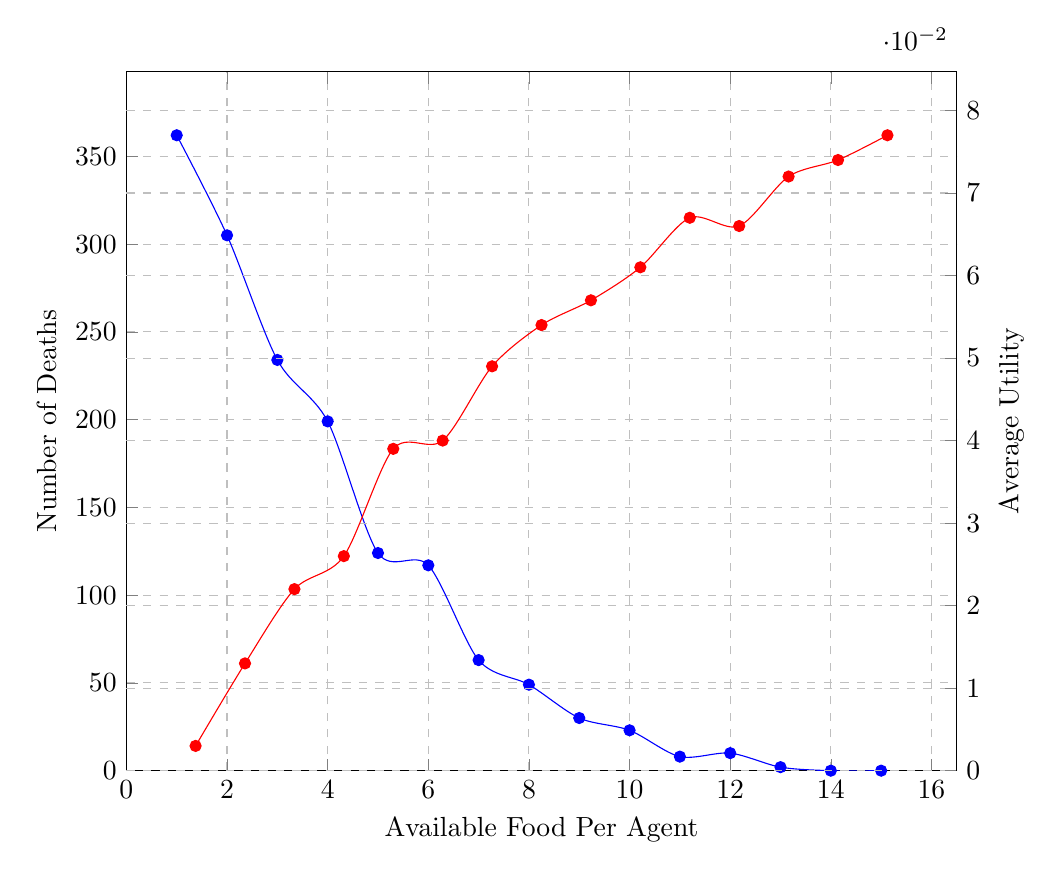
\begin{tikzpicture}
            \begin{axis}[
                width=\textwidth,
                axis y line*=left,
                ymin=0,
                xmin=0,
                xlabel=Available Food Per Agent,
                ylabel=Number of Deaths,
                ymajorgrids=true,
                xmajorgrids=true,
                grid style=dashed,
            ]
            \addplot[smooth,mark=*,blue]
                coordinates{
                    (15, 0)
                    (14, 0)
                    (13, 2)
                    (12, 10)
                    (11, 8)
                    (10, 23)
                    (9, 30)
                    (8, 49)
                    (7, 63)
                    (6, 117)
                    (5, 124)
                    (4, 199)
                    (3, 234)
                    (2, 305)
                    (1, 362)
                };
            \end{axis}
            
            \begin{axis}[
                width=\textwidth,
              axis y line*=right,
              axis x line=none,
              ymin=0,
              ylabel=Average Utility,
              ymajorgrids=true,
              xmajorgrids=true,
              grid style=dashed,
            ]
            \addplot[smooth,mark=*,red]
                coordinates{
                    (15, 0.077)
                    (14, 0.074)
                    (13, 0.072)
                    (12, 0.066)
                    (11, 0.067)
                    (10, 0.061)
                    (9, 0.057)
                    (8, 0.054)
                    (7, 0.049)
                    (6, 0.04)
                    (5, 0.039)
                    (4, 0.026)
                    (3, 0.022)
                    (2, 0.013)
                    (1, 0.003)
                };
            \end{axis}
            \end{tikzpicture}
    \end{minipage}
    \caption{Number of Deaths and Average Utility vs Available Food Per Agent}
    \label{fig:team5-deaths-utility-food-per-agent}
\end{figure}


















\section{Conclusion}\label{sec:team5-conclusion}





